\section{Исследование способов проектирования модульных систем}

При разработке высокопроизводительного фреймворка был 
использован язык программирования C++ стандарта 2014 года по 
ряду причин. Популярные интерпретируемые языки при разработке 
ядра системы не рассматривались из-за дополнительных затрат 
вычислительных ресурсов на интерпретацию кода. При разработке 
робототехнических систем активно используется низкоуровневое 
взаимодействие с аппаратной частью или с операционной системой 
поэтому для разработки программного обеспечания для РТК 
желательно использовать язык пригодный для системного 
программирования. Для решения подобных задач конкурентом 
C-подобным языкам является язык rust \cite{matsakis2014rust}, но 
на данный момент язык не имеет достаточного количество 
инструментов для разработки из-за чего от него пришлось 
отказаться. Язык С++ стандарта 2014 года имеет множество 
встроенных средств, позволяющих отказаться от использования 
библиотеки Boost. Boost – наиболее распространенная библиотека 
для расширения возможностей языка C++, включающая в себя 
огромное количество реализаций различных программных 
инструментов: от алгоритмов до метапрограммирования. 
Отказ от использования данной библиотеки позволит избавиться от 
большой зависимости и значительно облегчит платформу и ее 
развертывание. В языке C++ имеется встроенная поддержка 
многопоточности, что позволяет реализовать необходимые 
алгоритмы, такие как потокобезопасные контейнеры, управление 
многопоточным исполнением, синхронизация передаваемых данных и 
другие. Также с введением 11-го стандарта в языке C++ появилась 
поддержка ссылок на неименованные значения (rvalues), что 
позволяет использовать конструкторы перемещения вместо 
конструкторов копирования, значительно оптимизируя работу с 
памятью, что активно используется в работе.

Далее под модулем будет подразумеваться группа методов, которая 
принимает определенный набор данных и решает определенный набор 
задач независимо от конфигурации системы. Ядром системы является 
компонент, отвечающий за порядок исполнение модулей и задает 
фиксированный набор механизмов для коммуникации между ними. 
Каждый модуль может получать информацию о конфигурации системы и 
взаимодействовать с другими компонентами системы только через 
унифицированный интерфейс ядра.

\subsection{Примитивы межпоточной синхронизации}

Многопроцессное и многопоточное программирование является очень мощным инструментом для организации модульных приложений. Помимо хорошей масштабируемости такой подход позволяет эффективнее использовать возможности современных многоядерных аппаратных вычислительных устройств за счет одновременного исполнения различных частей кода.

В многопоточных системах часто возникает ситуация так называемой гонки за данные, когда два одновременно работающих потока обращаются к одной области памяти. В результате может нарушаться целостность данных, что приводит к ошибкам различного рода и которые тяжелло поддаются отладке. Для синхронизации данных существуют различные алгоритмы межпоточного взаимодействия. Условно алгоритмы можно разделить на две группы: блокирующие и неблокирующие. Блокирующие алгоритмы используют критические секции (mutex ) и примитивы, предоставляемые операционной системой. Неблокируюшие алгоритмы используют атомарные операции, которые доступны аппаратно, но существенно сложнее в разработке и проектировании.

% new
Вызовы функций операционной системы требуют перевода процессора 
из режима пользователя в режим ядра, что может существенно 
понизить общую производительность при частых обращениях. К таким 
вызовам относится в том числе и захват критической секции. В 
свою очередь атомарные операции позволяют синхронизировать 
обращение к данным за счет использования ресурсов процессора без 
обращения к ядру системы. Также обращения к ядру операционной 
системы предоставляют дополнительные трудности при использовании 
программного кода на других платформах и поэтому в ходе работы 
будет минимизироваться количество системных вызовов.

В данной работе исследование сконцентрированно на разработки модульной системы и коммуникации между модулями с искользованием lock-free алгоритмов. Как следует из названия, данные потокобезопасные контейнеры реализованы без использования мьютексов – взаимных исключений для обеспечения синхронизации при работе с несколькими потоками. Использование такого подхода позволяет значительно повысить скорость выполнения программы. Такие контейнеры соответствуют предполагаемой архитектуре программной платформы, поскольку в разрабатываемой платформе возможна ситуация MPMC (Multiple Producer Multiple Consumer) – данные в контейнер могут записываться из нескольких мест и считываться из нескольких мест. Использование контейнеров с блокирующей синхронизацией в таких случаях отрицательно сказывается на скорости работы программы при одновременном доступе к одной критической секции из разных потоков. Возможность применения таких контейнеров без использования сторонних библиотек обусловлена наличием необходимых для их реализации механизмов в 11-м стандарте языка С++.

В работе \cite{syzovalgorithm} рассматривается алгоритм для передачи большого количества данных через UDP-протокол в высоконагруженной многопоточной системе. В данной работе используется высокопроизводиетльная реализация очереди без блокировок с открытым исходным кодом <<moodycamel ConcurrentQueue>>, реализованная Камероном Десрочерзом (Cameron Desrochers). В данной работе предлагается использовать эту реализацию очереди для повышения быстройдействия в многопоточной среде. Ниже представленны графики тестирование производительности добавления элементов в очередь (рис. \ref{im:2_1_2_dequeue}) и получения элементов из очереди (рис. \ref{im:2_1_3_enqueue}), взятые с сайта разработчика. Тестирование производительности на процессоре Intel Atom z530 выдавало схожие соотношения результатов.

\begin{figure}[htb]
    \centering{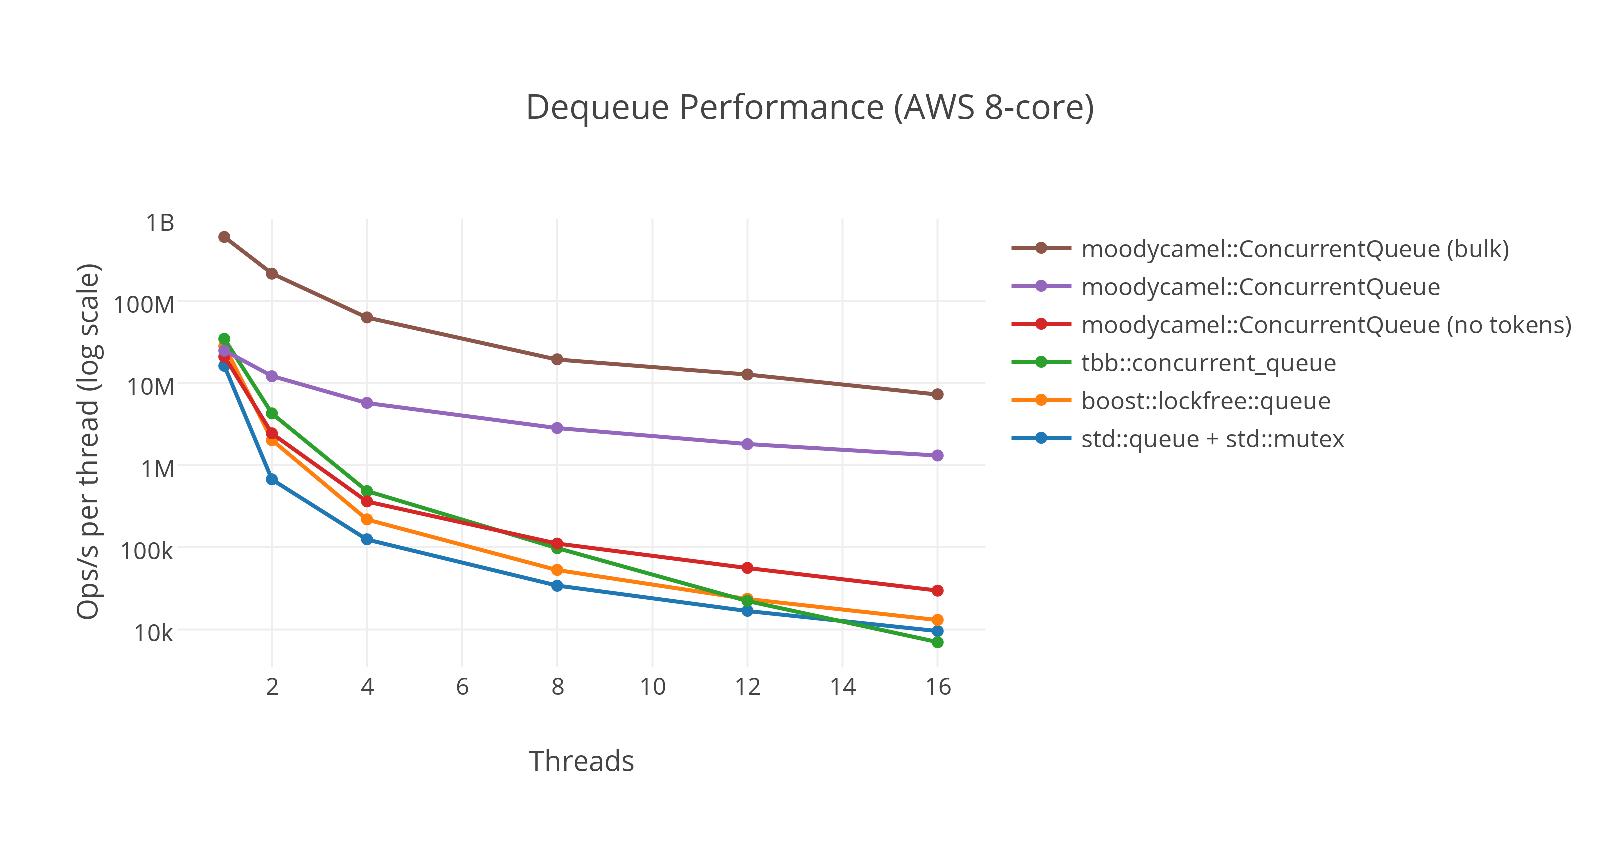
\includegraphics[width=1\linewidth]{2_1_2_dequeue}}
    \caption{Производительность получения элементов из очереди}
    \label{im:2_1_2_dequeue}
\end{figure}

\begin{figure}[htb]
    \centering{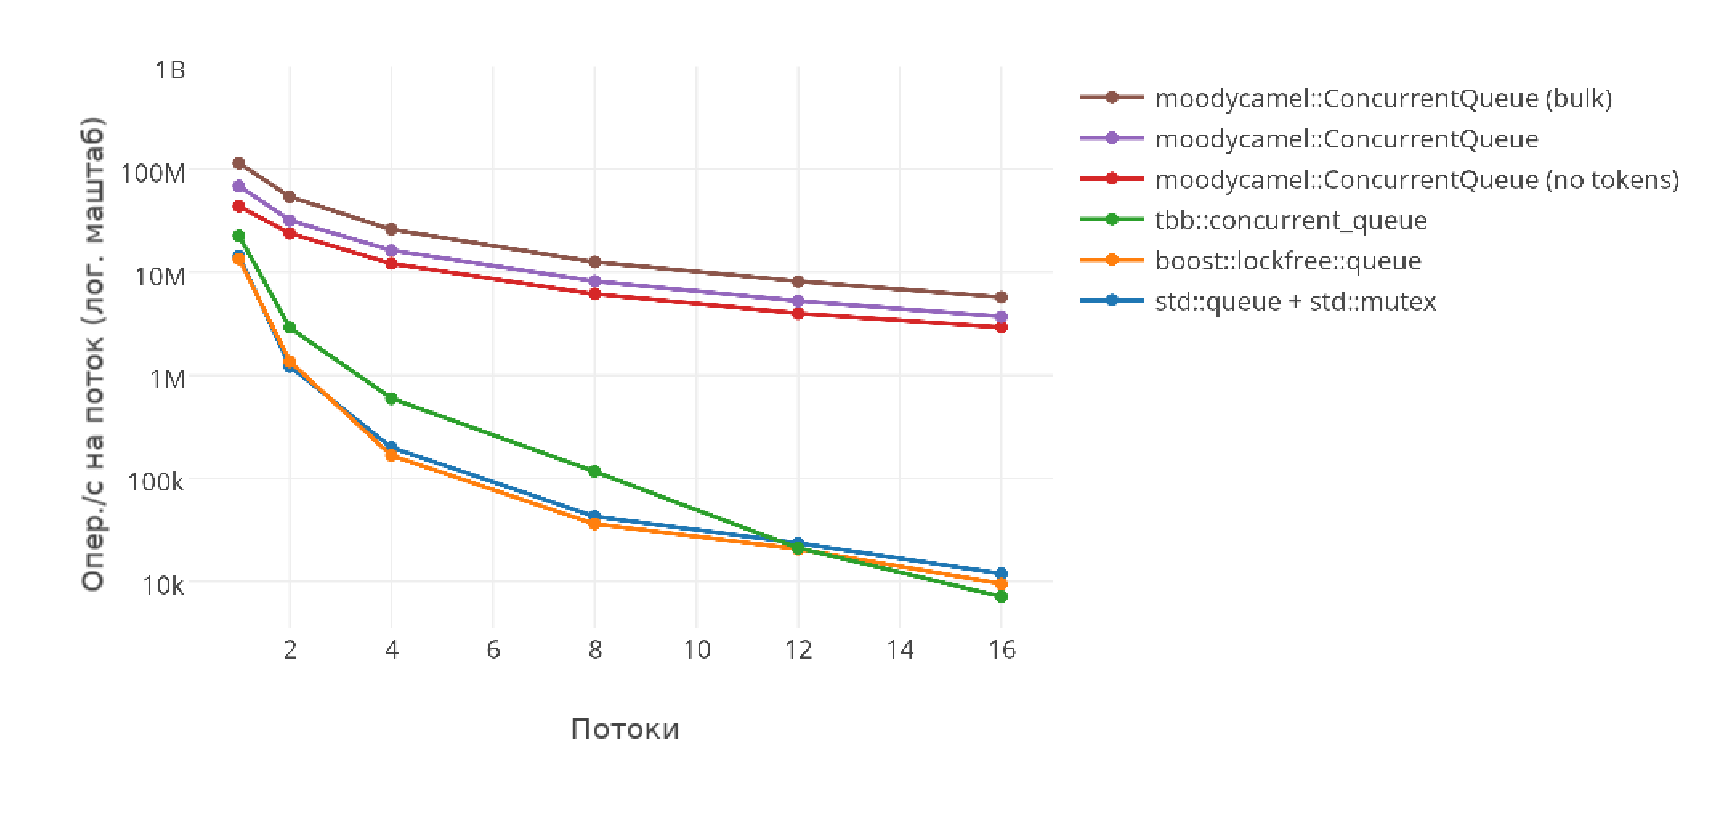
\includegraphics[width=1\linewidth]{2_1_3_enqueue}}
    \caption{Производительность добавления элементов в очередь}
    \label{im:2_1_3_enqueue}
\end{figure}

\subsection{Модели исполнения}

В данном разделе рассмотренны синхронные и асинхронные модели исполнения и проанализированны их слабые и сильные стороны при разработке модульных многопоточных приложений.

Современные стандарты языка C++ после введения шаблонов с переменным количеством типов (variadic templates) и лямбда-функций активно используют функциональные объекты и различные приемы, взятые из функциональных языков, которые позволяют существенно уменьшить количество классов при использовании стандартных шаблонов проектирования. Нововведения позволяют упростить разработку асинхронных приложений за счет использования высокоуровневых оберток вокруг функций и функциональных объектов (std::function). В основе реализации данного класса лежит паттерн type erasure. Его предназначение заключается в том, что различные сущности (объекты, указатели и пр.) скрываются за одним интерфейсом, которые предоставляют сходные возможности. Функциональный объект отвечает за хранение данных, поэтому имплементация интерфейса объекта создается и хранится в куче (heap). Узким местом такой реализации являются затраты на дополнительное аллоцирование памяти.

% Более подробное описание 

% Синхронная модель
В синхронном подходе требуется задать определенный интерфейс модуля, который будет последовательно выполнять определенную группу задач. Каждый модуль имеет входные точки: методы, в которых заключена вся логика обработки событий, полученных из ядра системы.

\begin{figure}[h]
    \centering{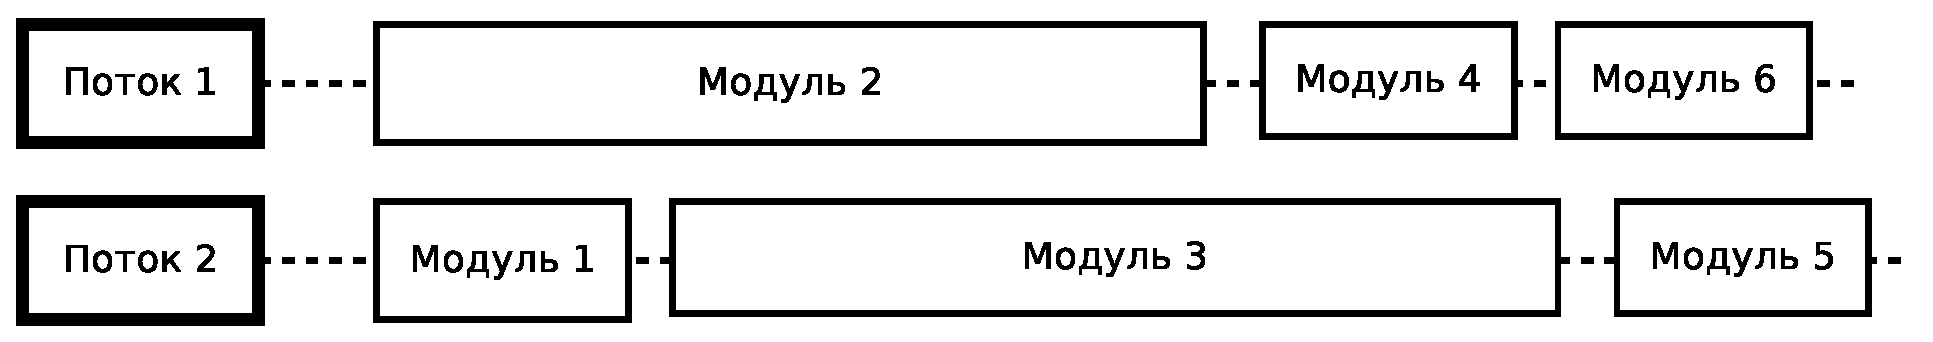
\includegraphics[width=1\linewidth]{2_1_1_sync}}
    \caption{Синхронное исполнение модулей в двух потоках}
    \label{im:2_1_1_sync}
\end{figure}

На рис. \ref{im:2_1_1_sync} изображена временная диаграмма обработки событий в двух потоках для синхронной системы. Этот график иллюстрирует типичную проблему данного подхода, когда несколько модулей имеют большое количество обработчиков входных данных (модули 2 и 3), из-за чего другие модули не имеют возможности продолжать обработку. Данная проблема может быть решена несколькими путями. В ROS данная проблема не возникает из-за того, что для каждого модуля создается отдельный процесс и используется системный планировщик задач для распределения нагрузки. Данный подход прямо зависит от реализации планировщика операционной системы, для которой разрабатывается фреймворк, а следовательно снижается переносимость кода. Другой вариант решения проблемы подразумевает, что разработчик модуля самостоятельно будет контролировать процессорное время, которое использует отдельный модуль, что существенно усложняет процесс разработки.

Так же синхронная модель исполнения подразумевает последовательную проверку входящих событий, что может привести к дополнительным вычислительным затратам при отсутствии входящих данных при большом количестве обработчиков событий.

При этом синхронный подход позволяет исключить гонку за данные 
при обновлении модулей в многопоточных системах, из-за чего 
можно не беспокоиться об обеспечении потокобезопасности при 
проектировании модуля, если ядро системы предоставляет такую 
модель исполнения.

% Асинхронная модель
Асинхронная модель исполнения предоставляет более гибкий способ разработки модулей. В основе данного подхода лежит отложенное исполнение кода и получение уведомлений о событиях в системе за счет функций обратного вызова. Каждый модуль можно разбить на цепочки небольших задач, которые добавляются в глобальную очередь и выполняются по мере выполнения других задач, что позволяет равномерно распределить процессорные ресурсы между потоками.

В данной работе ядро системы было реализованно с использованием как синхронного, так и асинхронного подхода для сравнения производительности и способов дальнейшего расширения функциональности системы.

\subsection{Алгоритмы сериализации}

При проектировании механизмов межмодульной коммуникации предполагается возможность использования системного ввода/вывода для взаимодействия с системой через сетевые протоколы или для записи сообщений на диск и повторного воспроизведения передаваемых данных в соответствующем порядке для отладки системы или иного сценария, подразумевающего подобное взаимодействие с операционной системой. Так же при проектировании учитывается возможность использовать компоненты и модули, реализованные на других языках программирования.

Данные при передаче между компонентами предполагается предавать 
в сериализированном виде. Это позволит обрабатывать данные на 
различных аппаратных архитектурах с разным порядком байт, 
различных языках программирования с использованием более 
эффективных структур для этого языка и передавать данные через 
сеть.

Сериализация - это процесс перевода какой-либо структуры данных в последовательность битов. Восстановление начальной структуры данных из сериализованной последовательности битов называется десериализацией.

В работе \cite{sumaray2012comparison} производится сравнение популярных форматов сериализации (XML, JSON, Protobuf, Thrift) при использовании на мобильных платформах. Из данной работы интерес представляют замеры производительности и объем потребляемой памяти для хранения структур данных. Результаты исследования показывают явное преимущество в этих двух аспектах у бинарных форматов сериализации Protobuf и Thrift. Человекочитаемые форматы XML и JSON позволяют упростить отладку системы, но из-за их избыточности в данной работе дальше рассматриваться не будут и дальнейшее исследование будет направленно в сторону бинарных форматов представления данных.

В работе \cite{zaluzhnyi2016serialization} исследуются алгоритмы сериализации и десериализации для высокопроизводительных вычислительных систем. Самые лучше результаты производительности показывают реализации Cap'n Proto и Google Flat Buffers, которые используют алгоритмы десериализации без копирования (zero-copy deserialization). Поскольку десериализация занимает пренебрежимо малое процессорное время, данные в таком формате можно передавать внутри системы сразу в сериализованном виде.

В связи с отсутствием зависимостей и поддержки большого количества языков (C, С++, Java Python, Go, JavaScript) и платформ  в данной работе при проектировании систем обмена сообщениями будет использованны реализации Protocol Buffers и Flat Buffers. В этих решениях каждая структура данных описывается в отдельном файле (schema) на специальном языке разметки. Для генерации програмнного кода для описанных структур используется сторонняя утилита соответствующая каждой из библиотек. Google Protocol Buffers позиционируется как компактный (memory efficient) инструмент для сериализации и десерелиализации данных. Компактность достигается за счет использования varint-подобных алгоритмов сжатия для целых чисел. Google Flat Buffers проектировался как аналог Protocol Buffers с уклоном в эффективное использование памяти для повышения быстродействия в играх реального времени, которые. В результате сериализированные данные существенно уступают в компактности, но при этом скорость работы алгоритмов пренебрежительно мала, что повышает эффективность работы в приложениях реального времени, которые критичны к любым потерям в производительности.
% Наработки по сериализатору
